\chapter{Naive Solution}
\label{chap:naivesoln}

To compare the efficiency of our approach, we present a straightforward solution for processing Spatial Alarms in Obstucted Space. The naive approach is a straight forward approach with no safe region computation.  This approach searches for a new alarm in the known region as soon as the client changes it's position.


In Section~\ref{naiveview}, we give an overview of the naive solution. Section~\ref{naivealgo} presents the algorithm of the solution. In Subsections 4.2.1, 4.2.2, 4.2.3, and 4.2.4, we discuss the steps of the algorithm in detail. Finally Section~\ref{flxQ2} proposes the improvements of this algorithm to save computational cost and client-server communication overheard.

\vspace*{12pt}

\section{Overview}
\label{naiveview}
The naive algorithm has three steps, first it computes the known region for POIs , then it computes the known region for obstacles and then it sends the visibility graph for all the POIs to the client.lastly the client computes the answer on every location change of the user.



\begin{figure}[!htbp]
\centering
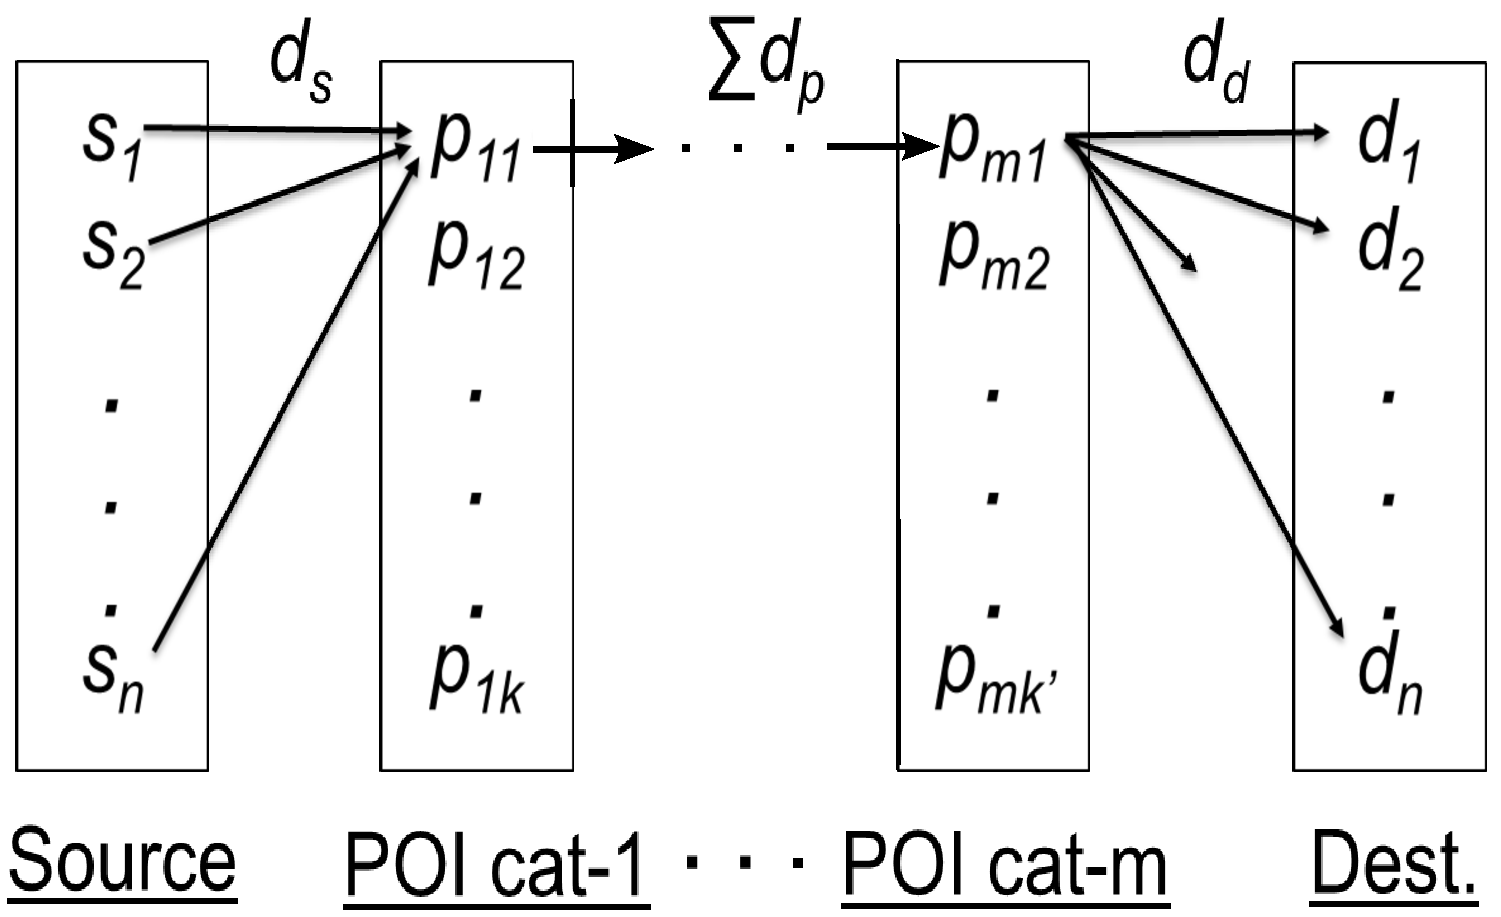
\includegraphics[width=0.7\columnwidth]{figures/soln1/naive.pdf}
\caption{Naive approach}
\label{fig:naive}
\end{figure}


\vspace*{12pt}

\section{Algorithm}
\label{naivealgo}

Algorithm~\ref{alg:gtpqna} shows the pseudocode for the naive approach for processing ordered $k$GTP queries. The input to the algorithms are the source location set \textit{S}, the destination set \textit{D}, the category set \textit{C}, the aggregate function to be minimized \textit{f} and \textit{k}. The output \textit{A} is $k$ sets of POIs that have $k$ smallest trip distances.

\vspace*{8pt}
We discuss the algorithm in the following four subsections. 

\begin{algorithm}
\caption{Initialization}
\label{Init}
\begin{algorithmic}[1]
\Procedure{Initialization}{}
\STATE incrementally increase r until it finds atleast 1 POI
\STATE Make
\STATE Retrieve all the obstacles inside the circular region of radius r$_kp$

\STATE r$_ko$ = r$_kp$
\STATE Construct the visibility graph V$_G$ for the POIs
\\ \While{there is any unreachable POI in the V$_G $ and there are more than 1 collision of obstacle perimeter of the circle of radius r$_ko$}
\State expand rko  until the unreachable POI gets reachable or there is less than 2 collisions
\State retrieve new obstacles;
\State If any new POI is found, then let r$_kp$ = r$_ko$ and go to the 3rd step
\EndWhile
\\Make O = {set of all obstacles inside the radius r$_ko$}
\\Return the client a response with  r$_kp$, r$_ko$, P, O 


\EndProcedure
\end{algorithmic}
\end{algorithm}





\subsection{$r_kp$ Computation}

The naive approach has two known regions, Known region for the POI and known region for the Obstacles. At first the known region for the POIs is computed. The radius of the known region is set to the alarming zone of the user upon initialization. The server, upon request of the client application, searches for POIs surrounding the user's current location. It incrementally increases the known regions radius, r$_kp$ until it finds atleast one POI. \\
\subsection{$r_ko$ computation}
\vspace*{5pt}
%\textbf{$\sum d_p$ Formulation:}
After computing r$_kp$ the server retrieves all the obstacles within this radius and sets the radius of the known region for obstacles,r$_ko$ as r$_kp$. Then it looks for any unreachable POIs within this region.The server incrementally increases r$_ko$ until all POIs are reachable.\\


\subsection{Visibility graph generation}
\vspace*{5pt}

\subsection{Recomputation on every location change}
\vspace*{5pt}
%\textbf{Exhaustive Search:}
Upon location change of the user the client application computes the obstructed distance from all the POI's in the known region and if any obstructed distance is less than the alarming distance, an alarm is invoked.





